% latexmk -shell-escape -pvc slides.tex # Watches and compiles on each change.
% latexmk -c slides.tex   # Clean the temporal files.

\documentclass[aspectratio=169]{beamer}

\setbeamertemplate{footline}[frame number]

\usepackage{caption}
\usepackage{graphicx}
\usepackage{hyperref}
\usepackage{siunitx}
\captionsetup[figure]{labelformat=empty}

\title{Use of time series of remote sensing imagery for Land Use monitoring}

\author{Alber S\'{a}nchez\\alber.ipia@inpe.br}
\institute{
  
\includegraphics[width=4cm,keepaspectratio]{logos/trees-color-h_2.png}
  
\includegraphics[width=1.8cm,keepaspectratio]
  {logos/logoinpe-azul-menor.png} \\
  Research assistant - TreesLab\\National Institute for Space Research - INPE\\
  Brazil
}
\date{2024-04-04}

\begin{document}

\frame{\titlepage}



\begin{frame}
    \frametitle{Overview}
    \tableofcontents
\end{frame}



%\section{Abstract}
%
%\begin{frame}
%    \frametitle{Abstract}
%    \small
%    Brazil is a country at the crossroads between environmental conservation and food production. On one hand, it is one of the largest producers of food, on the other, food production stresses what remains of its Biomes. To meet its international commitments, Brazil has to find an equilibrium between economic development and sustainable land management, articulated in  the form of policies and laws adapted and evolving with the reality of is territory.
%\newline
%\newline
%    At the same time, Remote Sensing is the most efficient way to monitor Land Use and Land Cover change (LULCC) over large extents. However, in its traditional form, it is constrained to relatively small spatio-temporal extents. This is due to factors such as the lack of access to the computational resources required to analyze the available sets of Earth Observation data.
%\newline
%\newline
%    During this presentation, we will show a summary of our experiences related to creating Land Use and Land Cover change maps in the Brazil Data Cube project. Where we were able to create exploratory LULCC maps using a mixture of modern classification techniques, large sets of time series data, and innovative computing platforms.
%\end{frame}
%
%\begin{frame}
%    \frametitle{Resumo}
%    \small
%O Brasil é um país na encruzilhada entre a conservação ambiental e a produção de alimentos. Por um lado, é um dos maiores produtores de alimentos, por outro, a produção de alimentos estressa o que resta dos seus Biomas. Para cumprir seus compromissos internacionais, o Brasil precisa encontrar um equilíbrio entre o desenvolvimento econômico e a gestão sustentável da terra, articulado na forma de políticas e leis adaptadas e evoluindo com a realidade do seu território. 
%\newline
%\newline
%Ao mesmo tempo, a Detecção Remota é a forma mais eficiente de monitorizar as alterações no Uso e Cobertura do Solo (LULCC) em grandes extensões. Contudo, na sua forma tradicional, está limitado a extensões espaço temporais relativamente pequenas. Isto se deve a fatores como a falta de acesso aos recursos computacionais necessários para analisar os conjuntos disponíveis de dados de Observação da Terra. 
%\newline
%\newline
%Durante esta apresentação, mostraremos um resumo de nossas experiências relacionadas à criação de mapas de mudança de uso e cobertura da terra no projeto Brazil Data Cube. Onde fomos capazes de criar mapas exploratórios LULCC usando uma mistura de técnicas modernas de classificação, grandes conjuntos de dados de séries temporais e plataformas computacionais inovadoras.
%\end{frame}



\section{Introduction}



\begin{frame}
    Introduction
\end{frame}



\begin{frame}
    \frametitle{Brazil is at a crossroad}
    \begin{columns}
        \begin{column}{0.5\textwidth}
            \begin{itemize}
                \item Food production versus environment 
                    conservation~\cite{garnett2011}.
                \item Brazil is one of the largest food producers. 
                \item Brazil hosts over ~60\% of Amazonia.
            \end{itemize}
        \end{column}
        \begin{column}{0.5\textwidth}
            \begin{figure}
                \centering
                
\includegraphics[width=0.9\textwidth]{img/crossroad.png}
                %\caption{Crossroad sign.}
                %\label{fig:crossroad_sign}
            \end{figure}
        \end{column}
    \end{columns}
\end{frame}



\begin{frame}
    \frametitle{Remote Sensing}
    \begin{columns}
        \begin{column}{0.5\textwidth}
            \begin{itemize}
                \item Remote Sensing is still the best way to water data about 
                    Land Use and Land Cover Change~\cite{picoli2018}.
                \item Traditionally, RS has been an human-expert intensive 
                    activity.
            \end{itemize}
        \end{column}
        \begin{column}{0.5\textwidth}
            \begin{itemize}
                \item Use of remote sensing imagery for conservation efforts. 
                \item Traditionally, remote sensing has focus on small areas.
                \item Pre-processing imagery is resource intensive.
            \end{itemize}
        \end{column}
    \end{columns}
\end{frame}



%\begin{frame}
%    \frametitle{Remote Sensing}
%    \begin{columns}
%        \begin{column}{0.5\textwidth}
%            \begin{itemize}
%                \item Multidimensional Data cubes take care of pre-processing 
%                    large amounts of satellite imagery~\cite{ferreira2020a}.
%                \item This enables user to run larger or more detailed studies.
%            \end{itemize}
%        \end{column}
%        \begin{column}{0.5\textwidth}
%        \end{column}
%    \end{columns}
%\end{frame}



\begin{frame}
    \frametitle{Analysis Ready Data}
    \begin{columns}
        \begin{column}{0.5\textwidth}
            \begin{itemize}
                \item Satellite data processed. 
                \item Allows immediate analysis. 
                \item Minimum user effort. 
                \item Interoperability through time. 
                \item Interoperability with other data 
                    sets~\cite{siqueira2019}.
            \end{itemize}
        \end{column}
        \begin{column}{0.5\textwidth}
            \begin{figure}
                \centering
                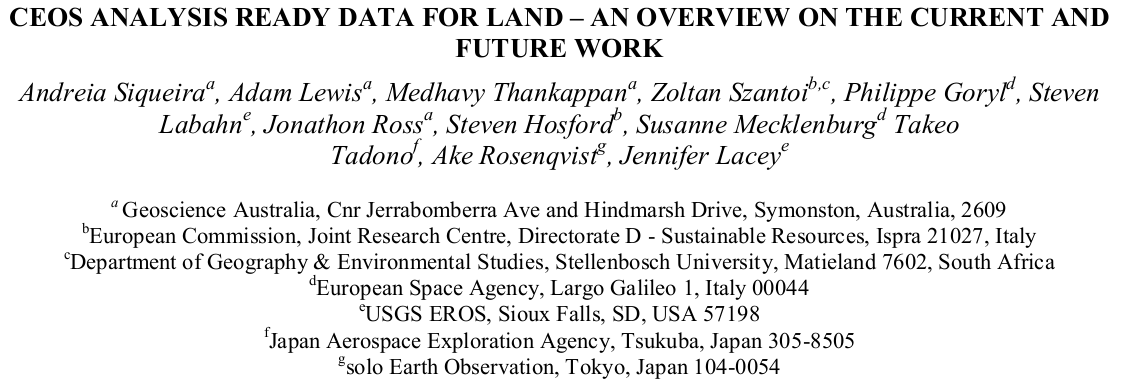
\includegraphics[width=0.9\textwidth]{img/siqueira2019.png}
            \end{figure}
        \end{column}
    \end{columns}
\end{frame}



\begin{frame}
    \frametitle{Data Cube}
    \begin{columns}
        \begin{column}{0.5\textwidth}
            \begin{itemize}
                \item A regular, dense, four-dimensional data 
                    structure~\cite{appel2019}.
                \item Data cube dimensions refer to the same spatial, temporal, 
                    and thematic reference systems.
                \item Data Cube cells have the same size and duration.
                \item Cells are aligned.
                \item A cell has a unique value.
            \end{itemize}
        \end{column}
        \begin{column}{0.8\textwidth}
            \begin{figure}
                \centering
                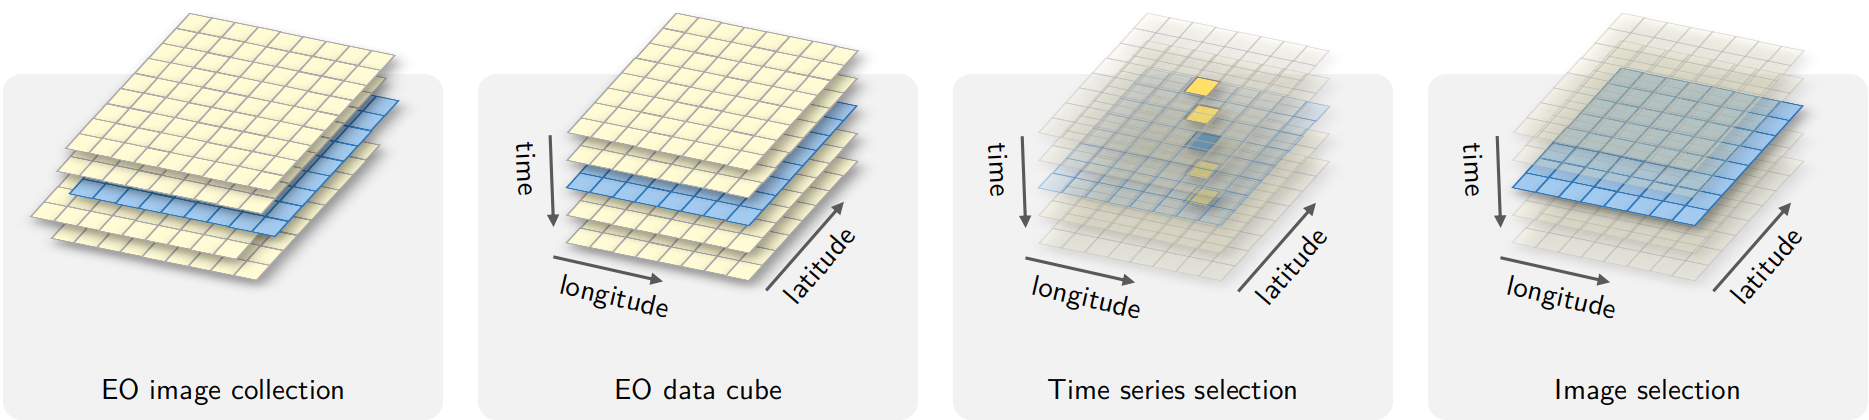
\includegraphics
                [width=0.6\textwidth,trim={7.8cm 0 15.7cm 0},clip]
                {img/datacube_conception.png}
                \caption{Source~\cite{gilbertocamara2023}.}
            \end{figure}
        \end{column}
    \end{columns}
\end{frame}



\begin{frame}
    \frametitle{Time series analysis}
    \begin{columns}
        \begin{column}{0.5\textwidth}
        \begin{itemize}
            \item Times series are experimental data observed at different 
                points in time.
            \item \emph{Time series analysis is a systematic approach by which 
                one goes about answering the mathematical and statistical 
                questions posed by time correlations}~\cite{shumway2017}.
        \end{itemize}
        \end{column}
        \begin{column}{0.5\textwidth}
            \begin{figure}
                \centering
                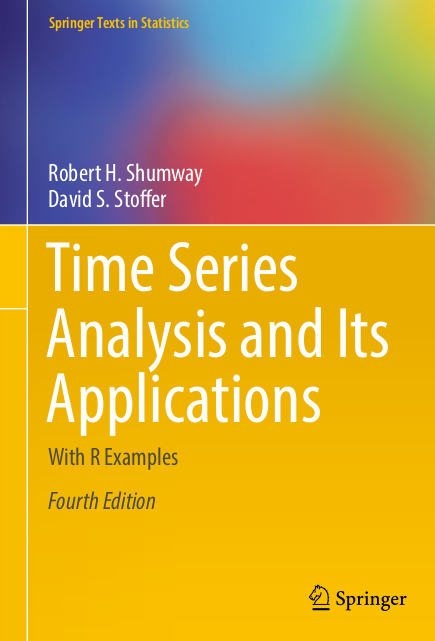
\includegraphics[width=0.6\textwidth]{img/shumway2017.png}
            \end{figure}
        \end{column}
    \end{columns}
\end{frame}



\begin{frame}
    \frametitle{Deep learning}
    \begin{columns}
        \begin{column}{0.5\textwidth}
            \begin{itemize}
                \item Artificial intelligence is the effort to automate 
                    intellectual tasks normally performed by humans.
                \item Machine Learning discovers rules to execute a 
                    data-processing task, given examples of what's expected.
                \item Deep Learning is a mathematical framework for learning
                    representations from data using successive layers of 
                    increasingly meaningful representations~\cite{chollet2018}.
            \end{itemize}
        \end{column}
        \begin{column}{0.5\textwidth}
            \begin{figure}
                \centering
                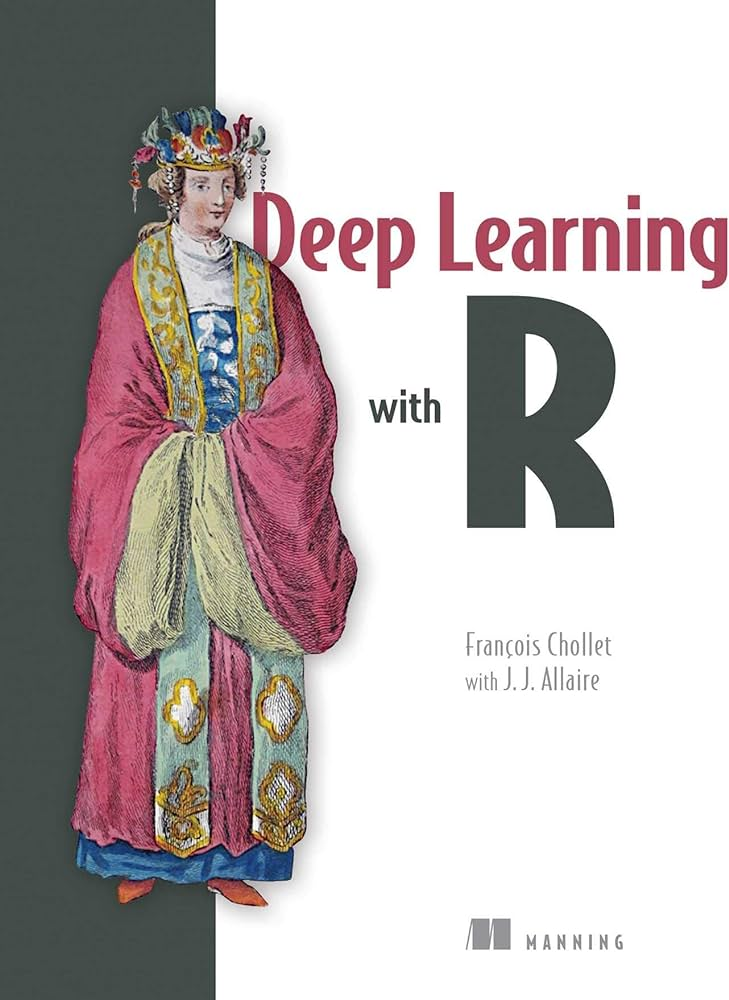
\includegraphics[width=0.6\textwidth]{img/chollet2018.jpg}
            \end{figure}
        \end{column}
    \end{columns}
\end{frame}





\section{Computing platforms}



\begin{frame}
    Computing platforms
\end{frame}



\begin{frame}
    \frametitle{Brazil Data Cube}
    \begin{columns}
        \begin{column}{0.5\textwidth}
            \begin{itemize}
                \item Production, visualization and analysis of large volumes 
                    of remote sensing images modeled as multidimensional data 
                    cubes for the entire Brazilian territory.
                \item Funded by FUNCATE. 
                \item Executed by INPE.
            \end{itemize}
        \end{column}
        \begin{column}{0.5\textwidth}
            \begin{figure}
                \centering
                
\includegraphics[width=0.5\textwidth]
                {img/brazil_data_cube_logo.png}
                \caption{}
                \label{}
            \end{figure}
        \end{column}
    \end{columns}
\end{frame}



\begin{frame}
    \frametitle{BDC architecture}
    \begin{figure}
        \centering
        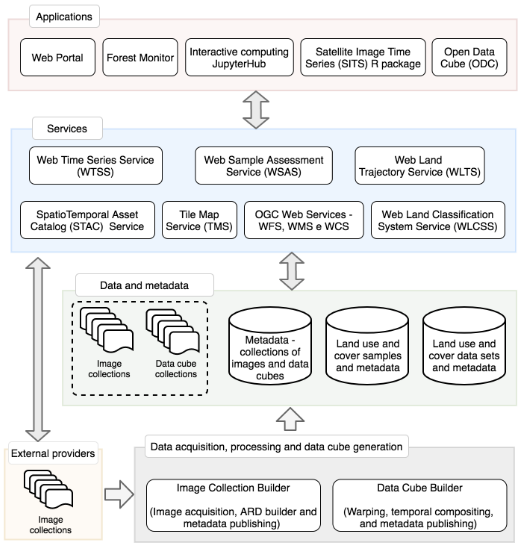
\includegraphics[width=0.45\textwidth]
        {img/brazil_data_cube_architecture.png}
        \caption{Brazil Data Cube architecture. Source~\cite{ferreira2020a}.}
        \label{fig:brazil_data_cube_architecture}
    \end{figure}
\end{frame}



\begin{frame}
    \frametitle{BDC Analysis Ready Data}
    \begin{figure}
        \centering
        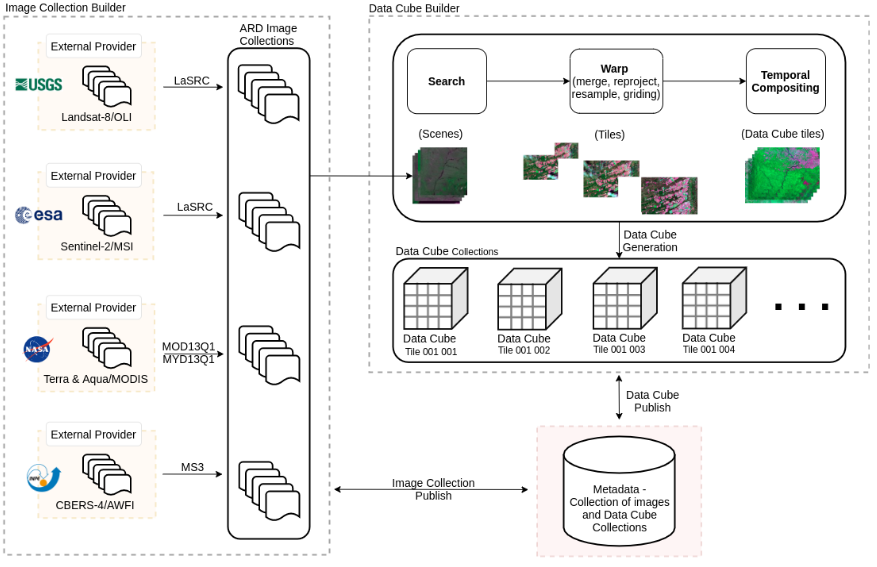
\includegraphics[width=0.75\textwidth]
        {img/analysis_ready_data_processing.png}
        \caption{Processing of Analysis Ready Data. 
        Source~\cite{ferreira2020a}}.
        \label{fig:analysis_ready_data_processing}
    \end{figure}
\end{frame}



\begin{frame}
    \frametitle{BDC cube regularization}
    \begin{figure}
        \centering
        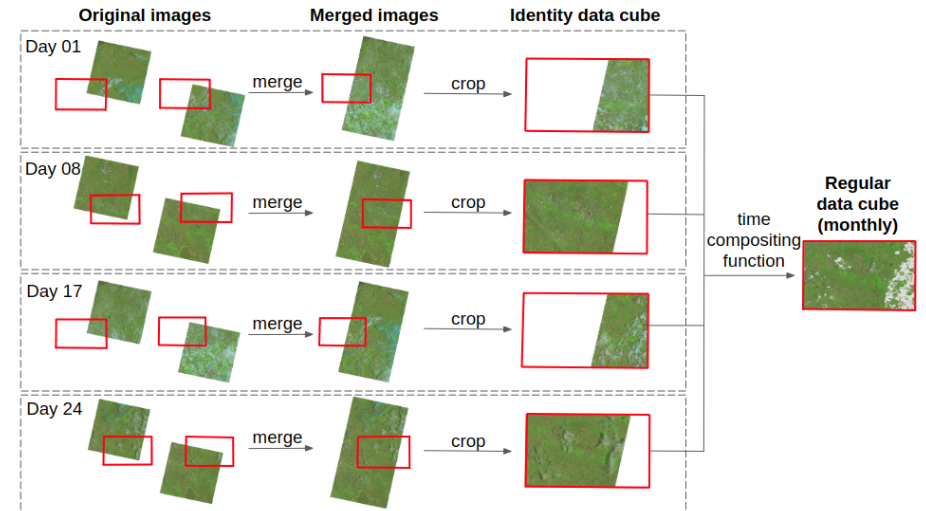
\includegraphics[width=0.85\textwidth]
        {img/brazil_data_cube_regularization.png}
        \caption{Imagery regularization into cubes. 
        Source~\cite{ferreira2020a}}.
        \label{fig:brazil_data_cube_regularization}
    \end{figure}
\end{frame}



\begin{frame}
    \frametitle{BDC cube composition}
    \begin{figure}
        \centering
        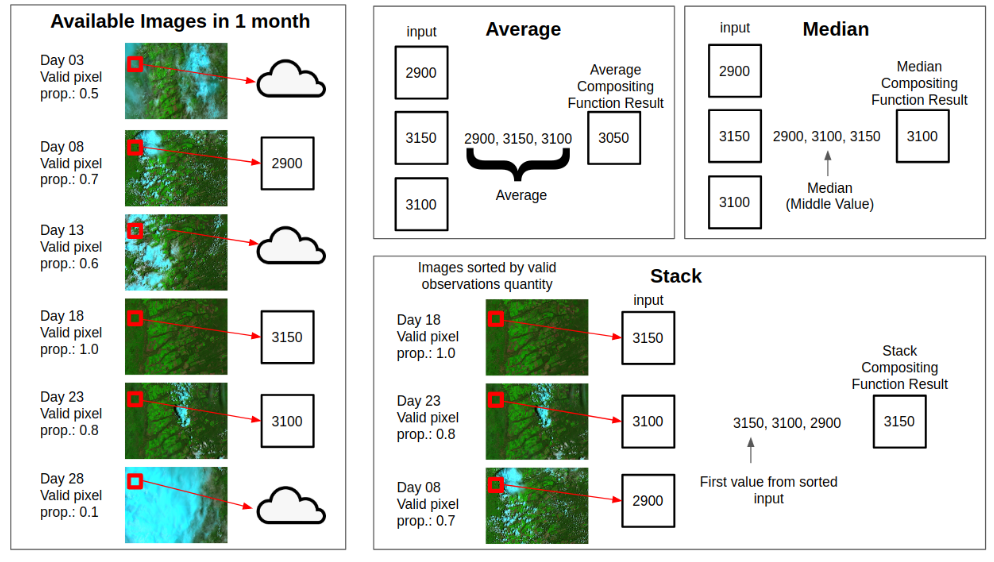
\includegraphics[width=0.85\textwidth]
        {img/brazil_data_cube_composition.png}
        \caption{Cube composition (cloud removal). 
        Source~\cite{ferreira2020a}}.
        \label{fig:brazil_data_cube_regularization}
    \end{figure}
\end{frame}



\section{Programming languages}



\begin{frame}
    Programming languages
\end{frame}

\begin{frame}
    \frametitle{The \emph{R} language}
    \begin{columns}
        \begin{column}{0.5\textwidth}
            \begin{itemize}
                \item \textit{R} language is a free software environment for 
                    statistical computing and graphics.
            \end{itemize}
        \end{column}
        \begin{column}{0.5\textwidth}
            \begin{figure}
                \centering
                
\includegraphics[width=0.5\textwidth]
                {img/Rlogo.png}
            \end{figure}
        \end{column}
    \end{columns}
\end{frame}



\begin{frame}
    \frametitle{\textit{R} \& Data Science}
    \begin{columns}
        \begin{column}{0.5\textwidth}
            \begin{itemize}
                \item \emph{Data science is an exciting discipline that allows 
                    you to transform raw data into understanding, insight, and 
                    knowledge}~\cite{wickham2023}.
            \end{itemize}
        \end{column}
        \begin{column}{0.5\textwidth}
            \begin{figure}
                \centering
                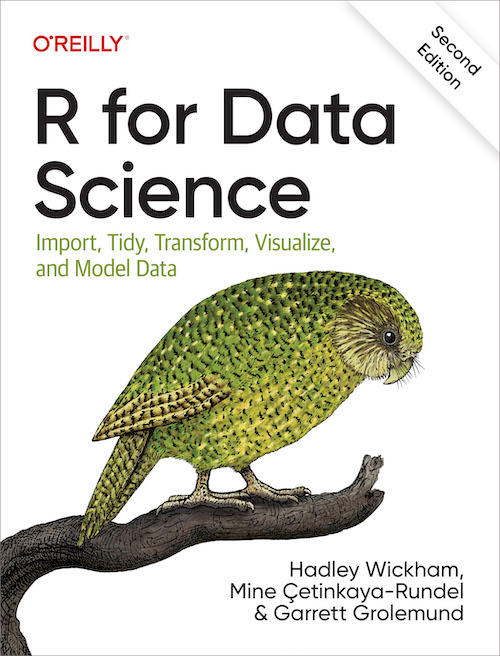
\includegraphics[width=0.7\textwidth]
                {img/wickham2023.jpg}
            \end{figure}
        \end{column}
    \end{columns}
\end{frame}



\begin{frame}
    \frametitle{The \emph{sits} package}
    \begin{columns}
        \begin{column}{0.5\textwidth}
            \begin{itemize}
                \item \emph{sits} stands for Satellite Image Time Series. 
                \item \emph{sits} is an open-source \textit{R} package for land 
                    use and land cover classification of big Earth observation 
                    data using satellite image time 
                    series~\cite{gilbertocamara2023}.
            \end{itemize}
        \end{column}
        \begin{column}{0.5\textwidth}
            \begin{figure}
                \centering
                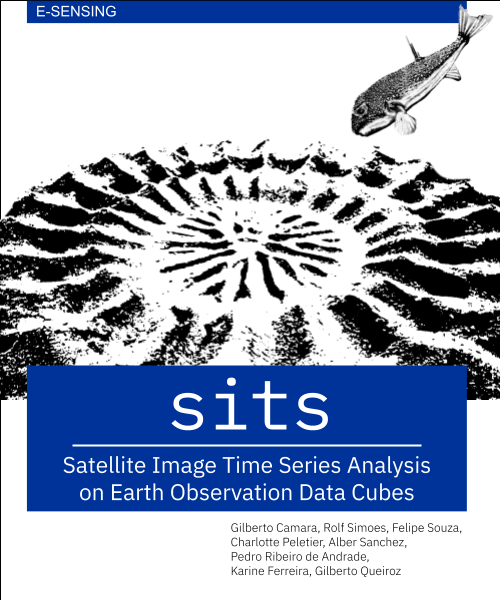
\includegraphics[width=0.7\textwidth]
                {img/sits_book.png}
            \end{figure}
        \end{column}
    \end{columns}
\end{frame}



\begin{frame}
    \frametitle{\emph{sits} overview}
    \begin{figure}
        \centering
        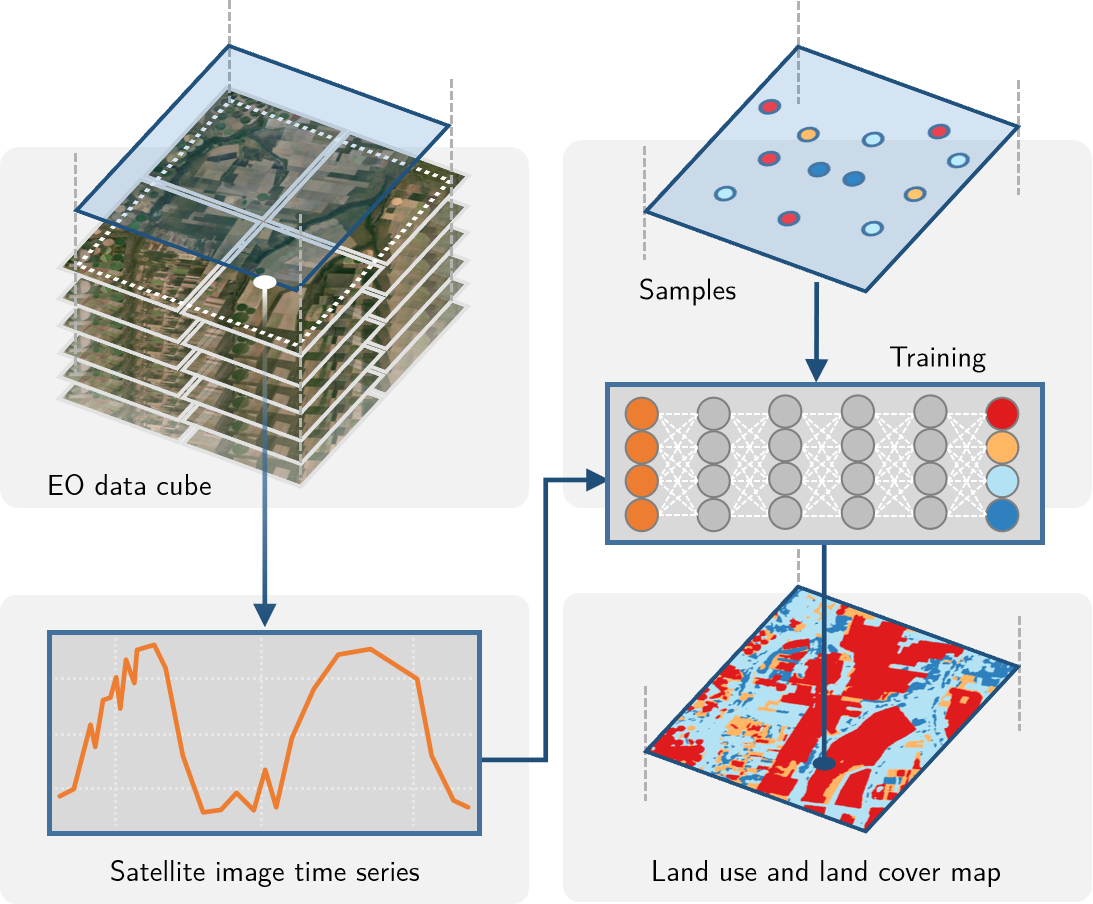
\includegraphics[width=0.55\textwidth]
        {img/sits_general_view.png}
        \caption{Source~\cite{gilbertocamara2023}.}
    \end{figure}
\end{frame}



\begin{frame}
    \frametitle{\emph{sits} main functions}
    \begin{figure}
        \centering
        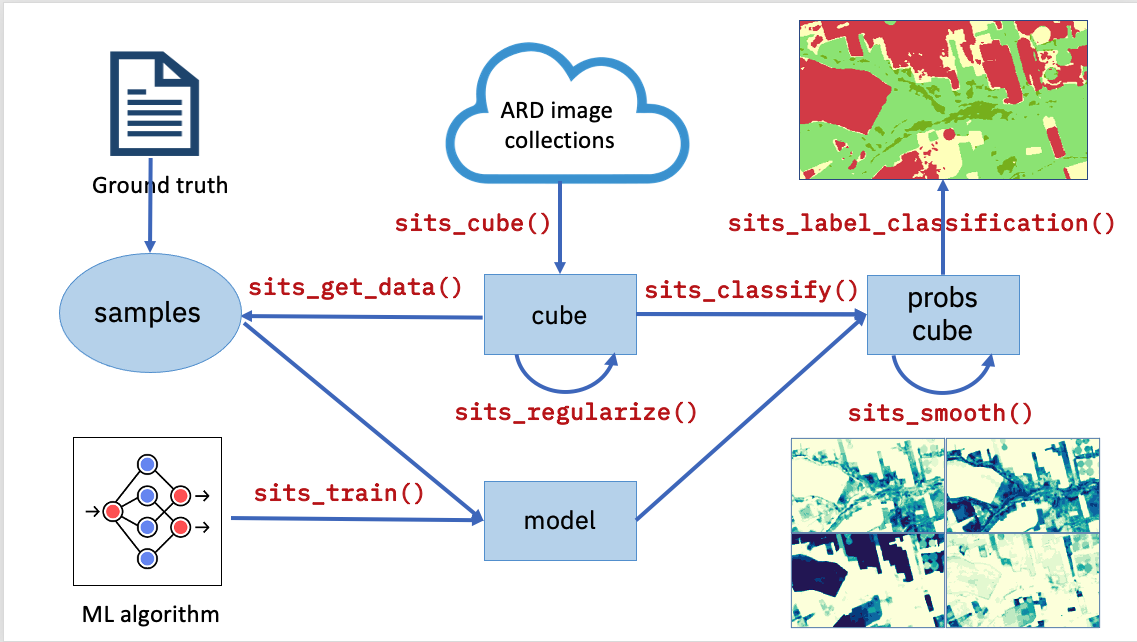
\includegraphics[width=0.8\textwidth]
        {img/sits_api.png}
        \caption{Source~\cite{gilbertocamara2023}.}
    \end{figure}
\end{frame}





\section{Results}



\begin{frame}
    Classifications of BDC Data Cubes
\end{frame}



\begin{frame}
    \frametitle{BDC Classifications}
    \begin{columns}
        \begin{column}{0.5\textwidth}
            \begin{itemize}
                \item Exploratory LULC maps of Braziilan Biomes. 
                \item Using R \& sits.
                \item Available online:\newline \scriptsize{\url{https://data.inpe.br/bdc/web/en/land-use-and-land-cover-classification/}}
            \end{itemize}
        \end{column}
        \begin{column}{0.5\textwidth}
            \begin{figure}
                \centering
                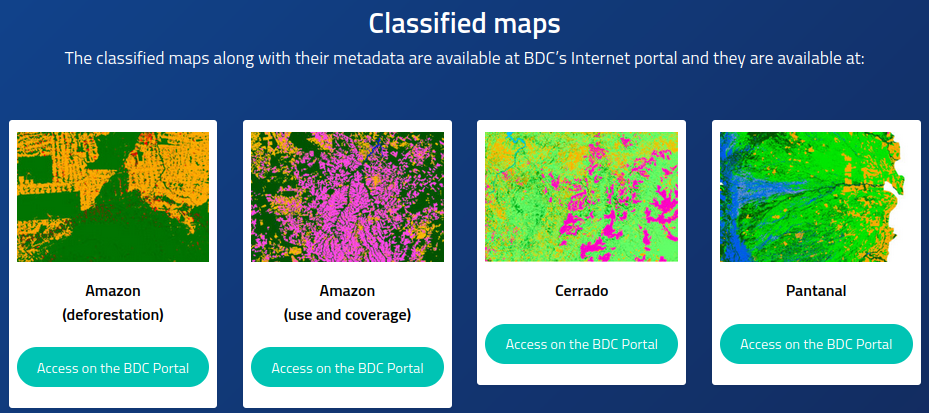
\includegraphics[width=0.9\textwidth]
                {img/brazil_data_cube_classifications.png}
            \end{figure}
        \end{column}
    \end{columns}
\end{frame}



\begin{frame}
    \frametitle{BDC Classification code}
    \begin{columns}
        \begin{column}{0.5\textwidth}
            \begin{itemize}
                \item R packages with code and samples, available 
                    online:\newline
                    \scriptsize{\url{https://github.com/brazil-data-cube/bdcclassifications}}
            \end{itemize}
        \end{column}
        \begin{column}{0.5\textwidth}
            \begin{figure}
                \centering
                
\includegraphics[width=0.7\textwidth]
                {img/r-packages.png}
            \end{figure}
        \end{column}
    \end{columns}
\end{frame}



\section{Conclusions}


\begin{frame}
    \frametitle{Conclusions}
    \begin{itemize}
        \item Classification of time series of Remote Sensing imagery is an 
            alternative to traditional way to produce Land Use Land Cover 
            Change (LULCC) maps. These maps are required for solving Brazil's 
            current crossroad between food production and environment 
            conservation.
        \item Open Source data and tools such as Brazil Data Cube and the 
            \emph{sits} package reduce the barriers to newcomers to LULCC 
            knowledge field.
        \item Exploratory LULCC maps of the Brazilian biomes are available 
            along with the platform, tools, and data required for their 
            improvement.
    \end{itemize}
\end{frame}



%----- References ----

\begin{frame}[allowframebreaks]
    \frametitle{References}
    \bibliographystyle{apalike}
    \bibliography{bibliography}
\end{frame}

\end{document}
